% =====================================================================
%  Algorithms_Report.tex -- SIMPLE team guide to the algorithms.
%  (The detailed version is Algorithms_Report_Detailed.tex/pdf.)
%  Build: tectonic Algorithms_Report.tex
% =====================================================================
\documentclass[11pt,a4paper]{article}
% =====================================================================
%  report_preamble.tex -- shared preamble for the stand-alone
%  Datasets and Algorithms reports (article class, A4).
% =====================================================================
\usepackage[T1]{fontenc}
\usepackage[utf8]{inputenc}
\usepackage{mathptmx}
\usepackage[a4paper,margin=2cm]{geometry}
\usepackage{amsmath,amssymb}
\usepackage{graphicx,xcolor}
\usepackage{tikz,pgfplots}
\pgfplotsset{compat=1.18}
\usetikzlibrary{positioning,arrows.meta,calc}
\usepackage{booktabs,array,multirow,tabularx,longtable}
\usepackage{pifont}
\providecommand{\checkmark}{\ding{51}}
\usepackage{enumitem}
\setlist{itemsep=1pt,topsep=3pt,parsep=0pt}
\usepackage[font=small,labelfont=bf]{caption}
\usepackage{float}
\usepackage{cite}
\usepackage{url}
\usepackage[colorlinks=true,linkcolor=hcBlue,citecolor=hcBlue,urlcolor=hcTeal]{hyperref}
\usepackage{titlesec}
\titleformat{\section}{\large\bfseries\color{hcBlue}}{\thesection}{0.6em}{}
\titleformat{\subsection}{\normalsize\bfseries}{\thesubsection}{0.6em}{}
\setlength{\parskip}{3pt}

% ---- Palette (colour-blind friendly) ----------------------------------
\definecolor{hcBlue}{HTML}{2166AC}
\definecolor{hcTeal}{HTML}{1B9E77}
\definecolor{hcOrange}{HTML}{D95F02}
\definecolor{hcPurple}{HTML}{7570B3}
\definecolor{hcRed}{HTML}{B2182B}
\definecolor{hcGray}{HTML}{6E6E6E}
\definecolor{boxBg}{HTML}{EEF3FA}

\pgfplotsset{
  hcaxis/.style={
    tick align=outside, tick pos=left, grid=major,
    major grid style={line width=0.2pt,draw=gray!30},
    axis line style={draw=gray!55},
    label style={font=\footnotesize},
    tick label style={font=\scriptsize},
    legend style={font=\scriptsize,draw=gray!40,fill=white,rounded corners=1pt},
    every node near coord/.append style={font=\tiny},
  }
}

\newcolumntype{L}[1]{>{\raggedright\arraybackslash}p{#1}}
\newcolumntype{Y}{>{\raggedright\arraybackslash}X}

% Highlight box for key take-aways
\newcommand{\keybox}[1]{%
  \par\smallskip\noindent\colorbox{boxBg}{\parbox{\dimexpr\linewidth-2\fboxsep}{\small #1}}\par\smallskip}

\setlength{\parindent}{0pt}

% A simple "algorithm card"
% #1 name, #2 used? tag, #3 simple idea, #4 why/why not, #5 paper link, #6 code link
\newcommand{\acard}[6]{%
\par\medskip\noindent
\colorbox{boxBg}{\parbox{\dimexpr\linewidth-2\fboxsep}{%
{\large\bfseries\color{hcBlue}#1}\hfill{\small #2}\\[3pt]
\begin{tabularx}{\linewidth}{@{}L{2.6cm} Y@{}}
\textbf{Simple idea} & #3 \\
\textbf{For our project} & #4 \\
\textbf{Paper} & \url{#5} \\
\textbf{Code} & \url{#6} \\
\end{tabularx}}}\par}
% Same card, but the "Code" field is plain text (no link)
\newcommand{\acardx}[6]{%
\par\medskip\noindent
\colorbox{boxBg}{\parbox{\dimexpr\linewidth-2\fboxsep}{%
{\large\bfseries\color{hcBlue}#1}\hfill{\small #2}\\[3pt]
\begin{tabularx}{\linewidth}{@{}L{2.6cm} Y@{}}
\textbf{Simple idea} & #3 \\
\textbf{For our project} & #4 \\
\textbf{Paper} & \url{#5} \\
\textbf{Code} & #6 \\
\end{tabularx}}}\par}

\newcommand{\used}{\colorbox{hcTeal!25}{\textbf{WE USE THIS}}}
\newcommand{\base}{\colorbox{hcBlue!15}{\textbf{BASELINE}}}
\newcommand{\info}{\colorbox{gray!20}{\textbf{GOOD TO KNOW}}}

\title{\color{hcBlue}\bfseries Algorithms: Simple Guide for the Team}
\author{Project: Skin Cancer Detection Using Deep Learning}
\date{}

\begin{document}
\maketitle
\vspace{-8mm}

\section*{1. What does our model have to do?}
Look at a skin photo and answer two questions:
\begin{enumerate}
  \item \textbf{Where is the lesion?} This is called
        \emph{segmentation}: drawing an outline around the spot.
  \item \textbf{What is it?} This is called \emph{classification}:
        choosing one of 8 labels, e.g., melanoma, BCC, or harmless mole.
\end{enumerate}

\section*{2. Words you need to know}
\begin{tabularx}{\linewidth}{@{}L{3.8cm} Y@{}}
\toprule
\textbf{Word} & \textbf{Simple meaning} \\
\midrule
Neural network / model & A program that learns patterns from examples instead of being told the rules \\
Training & Showing the model thousands of labelled photos so it learns \\
CNN & A model that scans the photo with small windows to find edges, colours, and textures \\
Transformer & A model that cuts the photo into small squares and compares every square with every other square to see the big picture \\
Pre-trained & A model that has already learned general images (dogs, cars, \ldots) from ImageNet; we then teach it skin photos. This saves a lot of time and data \\
Ensemble & Several models vote together, like asking three doctors instead of one \\
Parameters & The ``knobs'' inside a model. More knobs = bigger and slower model \\
Accuracy & Percentage of photos the model gets right \\
Balanced accuracy & Accuracy averaged over each class, so rare cancers count as much as common moles \\
Sensitivity & Out of all real cancers, how many did the model catch? (Most important for us) \\
\bottomrule
\end{tabularx}

\section*{3. Our pipeline in one picture}
\begin{center}
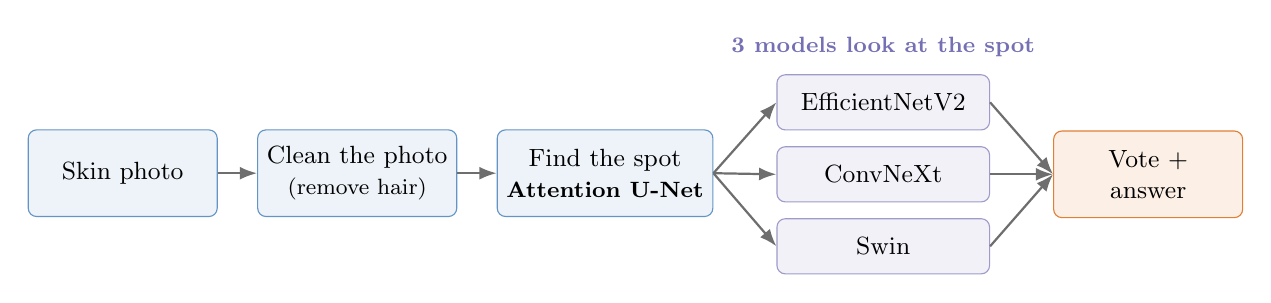
\begin{tikzpicture}[font=\small, node distance=4mm and 5mm,
  st/.style={draw=hcBlue!70,fill=hcBlue!8,rounded corners=3pt,minimum width=24mm,minimum height=11mm,align=center},
  md/.style={draw=hcPurple!70,fill=hcPurple!10,rounded corners=3pt,minimum width=27mm,minimum height=7mm,align=center},
  ot/.style={draw=hcOrange!80,fill=hcOrange!10,rounded corners=3pt,minimum width=24mm,minimum height=11mm,align=center},
  fl/.style={-{Latex[length=2.2mm]},draw=hcGray,thick}]
\node[st] (a) {Skin photo};
\node[st,right=of a] (b) {Clean the photo\\\footnotesize(remove hair)};
\node[st,right=of b] (c) {Find the spot\\\footnotesize\textbf{Attention U-Net}};
\node[md,right=8mm of c,yshift=9mm] (d1) {EfficientNetV2};
\node[md,below=2mm of d1] (d2) {ConvNeXt};
\node[md,below=2mm of d2] (d3) {Swin};
\node[ot,right=8mm of d2] (e) {Vote +\\answer};
\draw[fl] (a)--(b); \draw[fl] (b)--(c);
\draw[fl] (c.east)--(d1.west); \draw[fl] (c.east)--(d2.west); \draw[fl] (c.east)--(d3.west);
\draw[fl] (d1.east)--(e.west); \draw[fl] (d2.east)--(e.west); \draw[fl] (d3.east)--(e.west);
\node[above=1mm of d1,font=\footnotesize\bfseries,text=hcPurple] {3 models look at the spot};
\end{tikzpicture}
\end{center}
The answer contains: the diagnosis, how sure the model is, a
\textbf{heatmap} (Grad-CAM) showing which part of the photo it looked
at, and whether the patient should see a doctor.

% =====================================================================
\section*{4. Algorithms we USE}

\acard{Attention U-Net (finds the lesion)}{\used}
{A U-shaped network: the first half shrinks the photo to understand it,
the second half grows it back to draw the outline. ``Attention'' tells it
to ignore healthy skin and hair.}
{Step 1. It draws the lesion outline so we can cut out the spot. It
outlined lesions better than the plain U-Net in a fair test.}
{https://arxiv.org/abs/1804.03999}
{https://github.com/qubvel-org/segmentation_models.pytorch}

\acard{EfficientNetV2 (model 1 --- a CNN)}{\used}
{A CNN designed to be accurate \emph{and} fast by growing its depth,
width, and image size in a balanced way.}
{EfficientNet models won two big skin-cancer competitions
(ISIC 2019 and 2020). Medium size (about 22M parameters).}
{https://arxiv.org/abs/2104.00298}
{https://github.com/huggingface/pytorch-image-models}

\acard{ConvNeXt (model 2 --- a modern CNN)}{\used}
{An older CNN (ResNet) redesigned with tricks borrowed from
transformers. It thinks like a transformer but runs like a CNN.}
{A group of ConvNeXt models gave the best reported result on the
8-class ISIC 2019 data.}
{https://arxiv.org/abs/2201.03545}
{https://github.com/facebookresearch/ConvNeXt}

\acard{Swin Transformer (model 3 --- a transformer)}{\used}
{A transformer that looks at the photo in small windows and then
shifts the windows, so it sees both small details and the whole shape.}
{CNNs are good at texture; Swin is good at overall shape and symmetry.
Because they make \emph{different} mistakes, voting together makes the
team stronger.}
{https://arxiv.org/abs/2103.14030}
{https://github.com/microsoft/Swin-Transformer}

\acardx{Focal loss (training trick)}{\used}
{A way of scoring mistakes that punishes the model more when it gets
\emph{rare} or \emph{hard} photos wrong.}
{Cancer photos are rare. Without this, the model would mostly learn
``harmless mole''. In one study it added about 9 points of accuracy.}
{https://arxiv.org/abs/1708.02002}
{A few lines of PyTorch (torchvision has a 2-class version: \texttt{sigmoid\_focal\_loss})}

\acard{Grad-CAM (explanation heatmap)}{\used}
{Colours the photo red where the model paid most attention.}
{Lets the doctor check that the model looked at the lesion, not at a
ruler or hair. Builds trust.}
{https://arxiv.org/abs/1610.02391}
{https://github.com/jacobgil/pytorch-grad-cam}

% =====================================================================
\section*{5. Algorithms we compare against (baselines)}
We also train these simpler, well-known models so we can \emph{prove}
our method is better.

\acard{ResNet-50}{\base}
{A CNN with ``shortcut'' connections that let it be very deep without
getting confused. The most common starting model.}
{Standard baseline. 25.6M parameters.}
{https://arxiv.org/abs/1512.03385}
{https://github.com/huggingface/pytorch-image-models}

\acard{DenseNet-121}{\base}
{Every layer passes its findings to all later layers, so information is
reused. Small (8M parameters).}
{Baseline; popular in skin-cancer papers.}
{https://arxiv.org/abs/1608.06993}
{https://github.com/huggingface/pytorch-image-models}

\acard{MobileNetV2}{\base}
{A tiny CNN built to run on mobile phones (3.5M parameters).}
{Baseline, and a candidate for a future phone app.}
{https://arxiv.org/abs/1801.04381}
{https://github.com/huggingface/pytorch-image-models}

\acard{DINOv2 (quick strong baseline)}{\base}
{A big model that learned from 142 million unlabelled images. We only
add a small final layer on top, so it is cheap to try.}
{Quick check of how far a ready-made model can go.}
{https://arxiv.org/abs/2304.07193}
{https://github.com/facebookresearch/dinov2}

% =====================================================================
\section*{6. Other algorithms (good to know)}
\begin{tabularx}{\linewidth}{@{}L{2.9cm} Y L{3.4cm}@{}}
\toprule
\textbf{Algorithm} & \textbf{Simple idea / why not our main choice} & \textbf{Paper} \\
\midrule
SVM / Random Forest & Old-style machine learning with hand-made features. Much weaker than deep learning & -- \\
VGG16 & Early simple CNN. Very big (138M parameters) for its accuracy & \href{https://arxiv.org/abs/1409.1556}{\nolinkurl{arxiv.org/abs/1409.1556}} \\
InceptionV3 & CNN with filters of several sizes; used in the famous 2017 Nature skin-cancer paper & \href{https://arxiv.org/abs/1512.00567}{\nolinkurl{arxiv.org/abs/1512.00567}} \\
Xception & Faster version of Inception & \href{https://arxiv.org/abs/1610.02357}{\nolinkurl{arxiv.org/abs/1610.02357}} \\
EfficientNet (V1) & Older version of EfficientNetV2 & \href{https://arxiv.org/abs/1905.11946}{\nolinkurl{arxiv.org/abs/1905.11946}} \\
ViT & The first image transformer. Needs a lot of data, so Swin is better for us & \href{https://arxiv.org/abs/2010.11929}{\nolinkurl{arxiv.org/abs/2010.11929}} \\
U-Net & The original outline model (Attention U-Net is its upgrade) & \href{https://arxiv.org/abs/1505.04597}{\nolinkurl{arxiv.org/abs/1505.04597}} \\
TransUNet & U-Net with a transformer. Scored lower than Attention U-Net in a fair test & \href{https://arxiv.org/abs/2102.04306}{\nolinkurl{arxiv.org/abs/2102.04306}} \\
UCTransNet & Another U-Net upgrade; slightly better but more complex & \href{https://arxiv.org/abs/2109.04335}{\nolinkurl{arxiv.org/abs/2109.04335}} \\
PanDerm & A huge skin ``foundation model'' (2025). Very strong but needs big computers & \href{https://github.com/SiyuanYan1/PanDerm}{\nolinkurl{github.com/SiyuanYan1/PanDerm}} \\
\bottomrule
\end{tabularx}

% =====================================================================
\section*{7. How the algorithms compare (one simple chart)}
\begin{center}
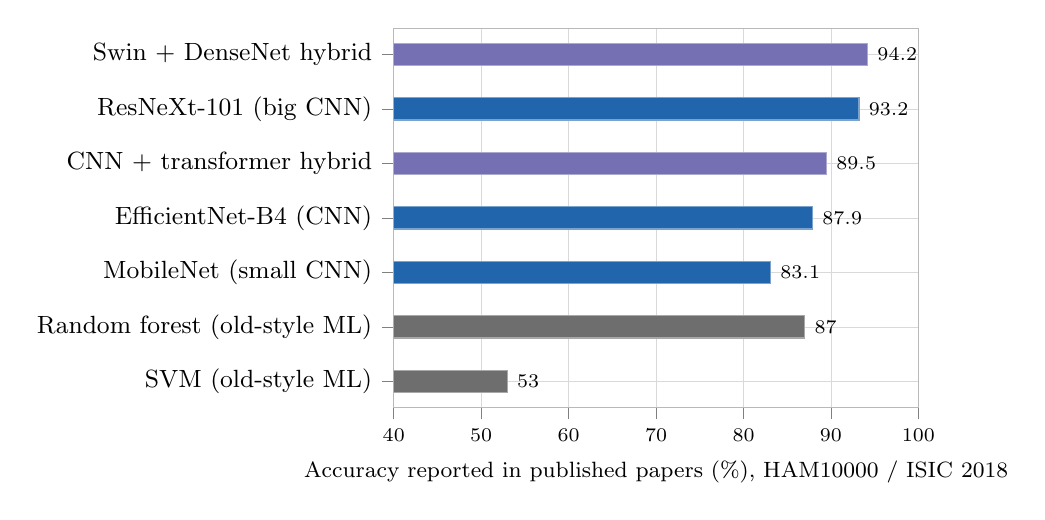
\begin{tikzpicture}
\begin{axis}[hcaxis,
  width=0.68\linewidth,height=6.4cm,
  xbar, bar width=8pt, bar shift=0pt,
  ytick={1,...,7},
  yticklabels={SVM (old-style ML),Random forest (old-style ML),MobileNet (small CNN),EfficientNet-B4 (CNN),CNN + transformer hybrid,ResNeXt-101 (big CNN),Swin + DenseNet hybrid},
  y tick label style={font=\small},
  xlabel={Accuracy reported in published papers (\%), HAM10000 / ISIC 2018},
  xmin=40,xmax=100, nodes near coords,
  every node near coord/.append style={font=\scriptsize},
  enlarge y limits=0.08]
\addplot[fill=hcGray,draw=hcGray!60] coordinates {(53,1)(87,2)};
\addplot[fill=hcBlue,draw=hcBlue!60] coordinates {(83.1,3)(87.9,4)(93.2,6)};
\addplot[fill=hcPurple,draw=hcPurple!60] coordinates {(89.5,5)(94.2,7)};
\end{axis}
\end{tikzpicture}
\end{center}
\keybox{\textbf{What the chart tells us:} deep learning is far better
than old-style machine learning, and mixing CNNs with transformers gives
the best results. \textbf{Careful:} these numbers come from different
papers with slightly different setups, so treat them as a rough guide.
Real-world results are usually lower. That is why we test on outside
datasets.}

% =====================================================================
\section*{8. Tools we will install}
\begin{tabularx}{\linewidth}{@{}L{3.4cm} L{5.2cm} Y@{}}
\toprule
\textbf{Tool} & \textbf{What for} & \textbf{Link} \\
\midrule
PyTorch & The main deep-learning library & \href{https://pytorch.org/}{\nolinkurl{pytorch.org}} \\
timm & Ready-made EfficientNetV2, ConvNeXt, Swin, ResNet, DenseNet, MobileNet & \href{https://github.com/huggingface/pytorch-image-models}{\nolinkurl{github.com/huggingface/pytorch-image-models}} \\
segmentation-models-pytorch & Ready-made U-Net for finding the lesion & \href{https://github.com/qubvel-org/segmentation_models.pytorch}{\nolinkurl{github.com/qubvel-org/segmentation_models.pytorch}} \\
pytorch-grad-cam & Heatmap explanations & \href{https://github.com/jacobgil/pytorch-grad-cam}{\nolinkurl{github.com/jacobgil/pytorch-grad-cam}} \\
scikit-learn & Data splitting and scores & \href{https://scikit-learn.org/}{\nolinkurl{scikit-learn.org}} \\
\bottomrule
\end{tabularx}

\keybox{\textbf{Summary:} Attention U-Net finds the spot $\rightarrow$
EfficientNetV2 + ConvNeXt + Swin each look at it $\rightarrow$ they vote
$\rightarrow$ we show the answer with a Grad-CAM heatmap. Focal loss
helps with rare cancers. ResNet-50, DenseNet-121, MobileNetV2, and DINOv2
are our baselines. The detailed version is in
\texttt{Algorithms\_Report\_Detailed.pdf}.}

\end{document}
